\documentclass[a4paper]{jacow}

\usepackage{mathtools}
\usepackage{amsmath}
\usepackage{xfrac}
\usepackage{xparse}
\usepackage{subcaption}
\usepackage{graphicx}
\usepackage{url}

\let\oldvec\vec
\renewcommand{\vec}{\boldsymbol}
\DeclareDocumentCommand{\bkt}{sm}{\IfBooleanTF{#1}{\left[ #2 \right]}{\left(#2\right)}}
\DeclareDocumentCommand{\ddt}{m}{\frac{\mathrm{d} {#1}}{\mathrm{d} t}}
\DeclareDocumentCommand{\pddx}{mO{t}O{}}{\frac{\partial^{#3} {#1}}{\partial {#2}^{#3}}}
\newcommand{\w}{\omega}
\newcommand{\W}{\Omega}
\newcommand{\subwidth}{.9\linewidth}
\newcommand{\D}{\Delta}

\begin{document}
\title{SPIN DECOHERENCE IN THE FROZEN SPIN STORAGE RING METHOD OF SEARCH FOR A PARTICLE EDM}
\author{A. E. Aksentyev\textsuperscript{1,2,3}\thanks{alexaksentyev@gmail.com},
  Y. V. Senichev\textsuperscript{3} \\
  \textsuperscript{1} National Research Nuclear University ``MEPhI,'' Moscow, Russia \\
  \textsuperscript{2} Institut f\"ur Kernphysik, Forschungszentrum J\"ulich, J\"ulich, Germany\\
  \textsuperscript{3} Institute for Nuclear Research of the Russian Academy of Sciences, Moscow, Russia}
\maketitle

\begin{abstract}
  Spin coherence refers to a measure of preservation of polarization in an initially polarized beam.
  The spin vector of a particle injected into a storage ring starts to precess about
  the vertical magnetic field vector in accordance with the Thomas-BMT equation. The precession frequency
  is dependent on the equilibrium-level energy, which differs across the beam particles.
  This does not pose a problem when the initial polarization is vertical; however,
  the Frozen Spin Storage Ring EDM search method requires beam polarization along the momentum vector,
  i.e., in the horizontal plane. 
  
  In the present work we analyze the source of decoherence, and investigate the way it can be suppressed
  in the horizontal plane in a perfectly aligned ring by means of sextupole fields. We also consider
  the case of an imperfect ring: transference of decoherence into the vertical plane induced by vertical
  plane spin precession, and the effect of sextupole fields.
\end{abstract}

\section{Spin dynamics in a storage ring}
The dynamics of a spin-vector $\vec s$ in a magnetic field $\vec B$ and an electrostatic field $\vec E$
is described by the Thomas-BMT equation. Its generalized version, accounting for the effect of
the particle's electric dipole moment, can be written in the rest frame as:
\begin{subequations}
  \begin{align}
    \ddt{\vec s} &= \vec s\times \bkt{\vec\W_{MDM} +\vec\W_{EDM}}, \label{eq:TBMT_main}
    \intertext{where the magnetic (MDM) and electric (EDM) dipole moment angular velocities
      $\vec\W_{MDM}$ and $\vec\W_{EDM}$ }
    \vec\W_{MDM} &= \frac qm \bkt*{G\vec B - \bkt{G - \frac{1}{\gamma^2-1}}\frac{\vec E\times\vec\beta}{c}},\label{eq:TBMT_MDM} \\
    \vec\W_{EDM} &= \frac qm \frac\eta2 \bkt*{\frac{\vec E}c + \vec\beta\times \vec B}.\label{eq:TBMT_EDM}
  \end{align}
\end{subequations}
In the above equations, $m,~q,~G=(g-2)/2$ are, respectively, the mass, charge, and anomalous magnetic moment
of the particle; $\beta = \dfrac{v_0}{c}$ is its normalized speed; $\gamma$ its Lorentz factor.
The EDM factor $\eta$ is defined by equation $d = \eta\frac{q}{2mc}$, in which $d$ is the particle EDM,
$s$ its spin.

In the standard formalizm one operates with the spin transfer matrix~\cite[p.~4]{COSY:SpinTuneMapping}
\[
\boldsymbol{t}_R = \exp\bkt{-i\pi\nu_s\vec\sigma\cdot\bar n} = \cos\pi\nu_s - i (\vec\sigma\cdot\bar n)\sin\pi\nu_s,
\]
where $\nu_s = \sfrac{\W_s}{\W_{cyc}}$, the ratio of the particle's spin precession frequency to
its cyclotron frequency, is termed \emph{spin tune}, and $\bar n$, termed the \emph{invariant spin axis},
defines the spin precession axis. They relate to the spin precession angular velocity as in
$\vec\W_s = \w_{cyc}\cdot \nu_s\bar n$.

\section{Origin of decoherence}
Spin decoherence in a particle beam is a result of the difference of the particles' spin precession
angular velocities ($\vec\W_s$), which, in turn, is caused by the difference of their orbit lengths.

The longitudinal dynamics of a particle on the reference orbit in a storage ring is described by
the system of equations:
\begin{equation}
  \begin{cases}
    \ddt{\D\varphi} &= -\w_{RF}\eta\delta, \\
    \ddt{\delta} &= \frac{q V_{RF}\w_{RF}}{2\pi h\beta^2E}\bkt{\sin\varphi - \sin\varphi_0}.
  \end{cases}
\end{equation}
In the equations above, $\D\varphi = \varphi-\varphi_0$ and  $\delta = (p-p_0)/p_0$ are the deviations
of the particle's phase and normalized momentum from those of the reference particle;
$V_{RF}$, $\w_{RF}$ are the amplitude and frequency of the RF field;
$\eta = \alpha_0 - \gamma^{-2}$ is the slip-factor, where $\alpha_0$ is
the momentum compaction factor defined by $\sfrac{\Delta L}{L} = \alpha_0\delta$, $L$ being the orbit length;
$h$ is the harmonic number; $E$ the total energy of the particle.

The solutions of this system form a family of ellipses in the $(\varphi, \delta)$-plane, all centered at the point
$(\varphi_0,\delta_0)$. However, if one considers a particle involved in betatron oscillations, and uses a
higher-order Taylor expansion of the momentum compaction factor $\alpha = \alpha_0 + \alpha_1\delta$,
the first equation of the system transforms into:~\cite[p.~2579]{Senichev:IPAC13-WEPEA036}
\[
\ddt{\varphi} = -\w_{RF} \bkt*{\bkt{\frac{\Delta L}{L}}_\beta + \bkt{\alpha_0 + \gamma^{-2}}\delta + \bkt{\alpha_1 - \alpha_0\gamma^{-2} + \gamma^{-4}}\delta^2},
\]
where $\bkt{\frac{\Delta L}{L}}_\beta = \frac{\pi}{2L}\bkt*{\varepsilon_xQ_x + \varepsilon_yQ_y}$, is
the betatron motion-related orbit lengthening; $\varepsilon_x$ and $\varepsilon_y$ are the
horizontal and vertical beam emittances, and $Q_x$, $Q_y$ are the horizontal and vertical tunes.

The solutions of the transformed system are no longer centered at the same single point.
Orbit lengthening and momentum deviation cause an equilibrium-level momentum shift~\cite[p.~2581]{Senichev:IPAC13-WEPEA036}
\begin{equation}\label{eq:EquLevMom_shift}
\Delta\delta_{eq} = \frac{\gamma_0^2}{\gamma_0^2\alpha_0 - 1}\bkt*{\frac{\delta_m^2}{2}\bkt{\alpha_1 - \alpha_0\gamma^{-2} + \gamma_0^{-4}} + \bkt{\frac{\Delta L}{L}}_\beta},
\end{equation}
where $\delta_m$ is the amplitude of synchrotron oscillations.

The equilibrium energy level, associated with the momentum shift~\eqref{eq:EquLevMom_shift},
termed the \emph{effective Lorentz factor}, is\cite{Senichev:2017amn}
\begin{equation}\label{eq:EffectiveGamma}
\gamma_{eff} = \gamma_0 + \beta_0^2\gamma_0\cdot\Delta\delta_{eq},
\end{equation}
where $\gamma_0$, $\beta_0$ are the Lorentz factor and normalized speed of the reference particle.

From the T-BMT equation~\eqref{eq:TBMT_MDM}, and the equation for cyclotron frequency in a magnetic field
$\w_{cyc} = \frac qm \frac B\gamma$, spin tune $\nu_s = \gamma_{eff}G$; therefore, the variation of
orbit lengths over the beam particles casues spin tune dispersion, and consequently --- spin decoherence.

\section{Sextupole field suppression of decoherence}
A sextupole field with gradient $ S_{sext} = \frac{1}{B\rho} \pddx{B_y}[x][2]$, has a twofold effect
on decoherence:
\begin{itemize}
\item it directly affects the particles' orbit lengths:
  $\bkt{\frac{\Delta L}{L}}_{sext} = \mp \frac{S_{sext}D_0\beta_{x,y}\varepsilon_{x,y}}{L}$, and
\item it modifies the lattice's momentum compaction factor: $\Delta \alpha_{1,sext} = -\frac{S_{sext}D_0^3}{L}$.
\end{itemize}
Above, $\beta_{x,y}$ are the horizontal, vertical beta-functions;
$D(s) = D_0(s) + D_1(s)\delta$ is the dispersion function; $B\rho$ is the magnetic rigidigy.

Consequently, in order to reduce decoherence associated with horizontal and vertical betatron oscillations,
and with synchrotron oscillations, correcting sextupoles must be placed, respectively, in the maxima of
the $\beta_x$-, $\beta_y$- and $D$-functions.
\section{Simulation of decoherence suppression}
In this simulation we used a Frozen Spin-type lattice shown in Fig.~\ref{fig:FSBNL_lattice}.
All optical elements are perfectly aligned, i.e., there's no spin precession about the
radial coordinate system axis. Particles were injected at 270 MeV kinetic energy, which is the
frozen spin energy for the deuteron in this lattice. Computations were performed using the
COSY INFINITY code.~\cite{COSY:Website} Spin tune and invariant spin axis Taylor expansions
were computed up to 5th order. Simulation results are presented in Fig.~\ref{fig:decoherence_suppression_sim}.

\begin{figure}[h!]
  \centering
  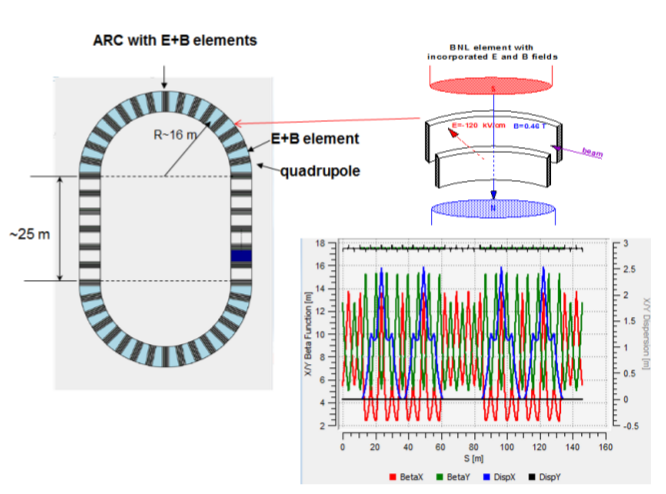
\includegraphics[width=\linewidth]{../img/Lattice/BNL}
  \caption{Frozen spin-type lattice used in simulations.\label{fig:FSBNL_lattice}}
\end{figure}
\begin{figure}[ht]
  \centering
  \begin{subfigure}{\subwidth}
    \centering
    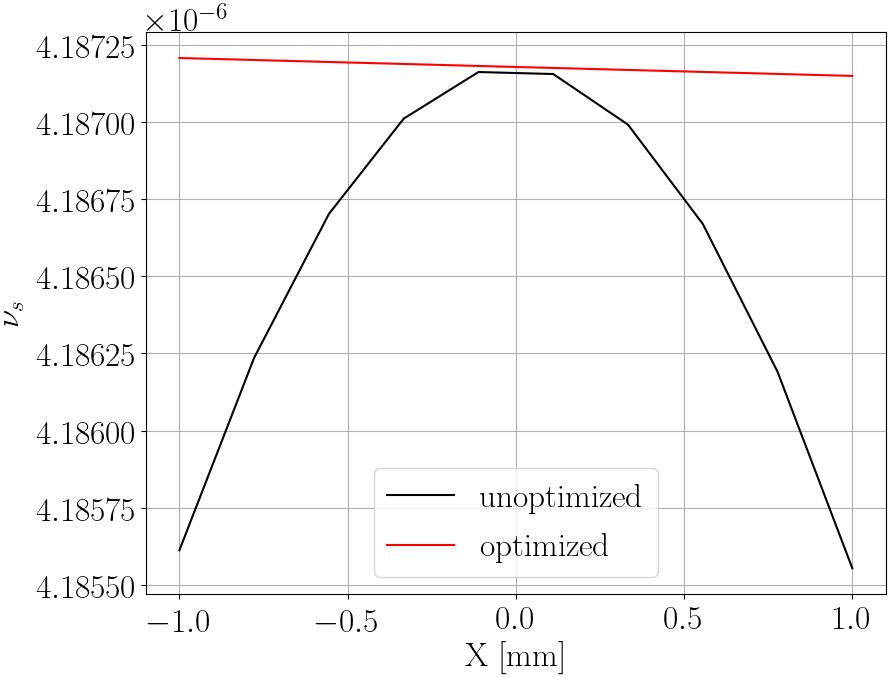
\includegraphics[width=\linewidth]{../img/IPAC19/spin_tune_decoh_x_offset}
    \caption{For particles involved in horizontal betatron oscillation only.\label{fig:st_decoh_horizontal}}
  \end{subfigure}
  \begin{subfigure}{\subwidth}
    \centering
    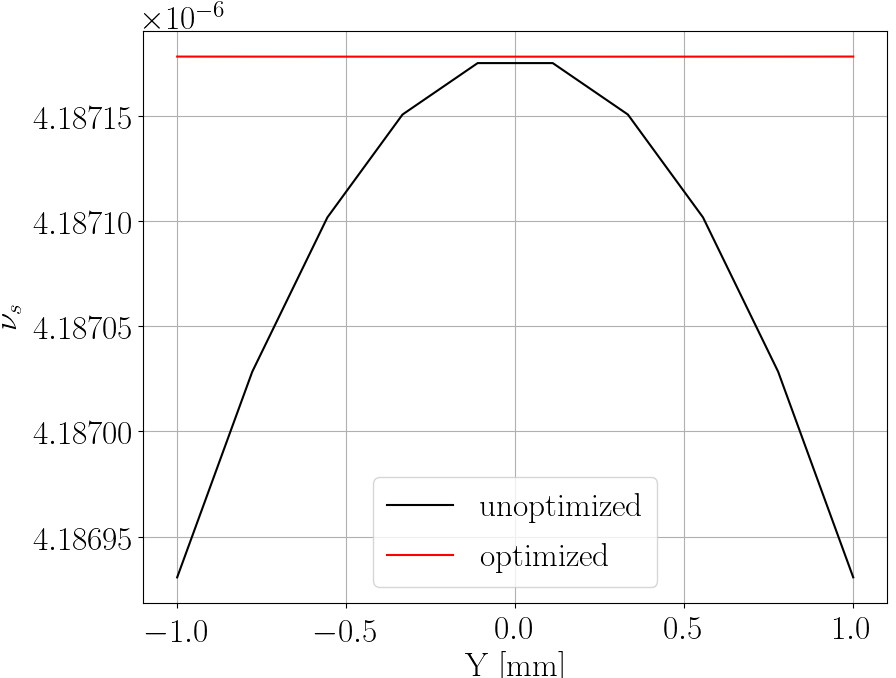
\includegraphics[width=\linewidth]{../img/IPAC19/spin_tune_decoh_y_offset}
    \caption{For particles involved in vertical betatron oscillation only.}
  \end{subfigure}
  \begin{subfigure}{\subwidth}
    \centering
    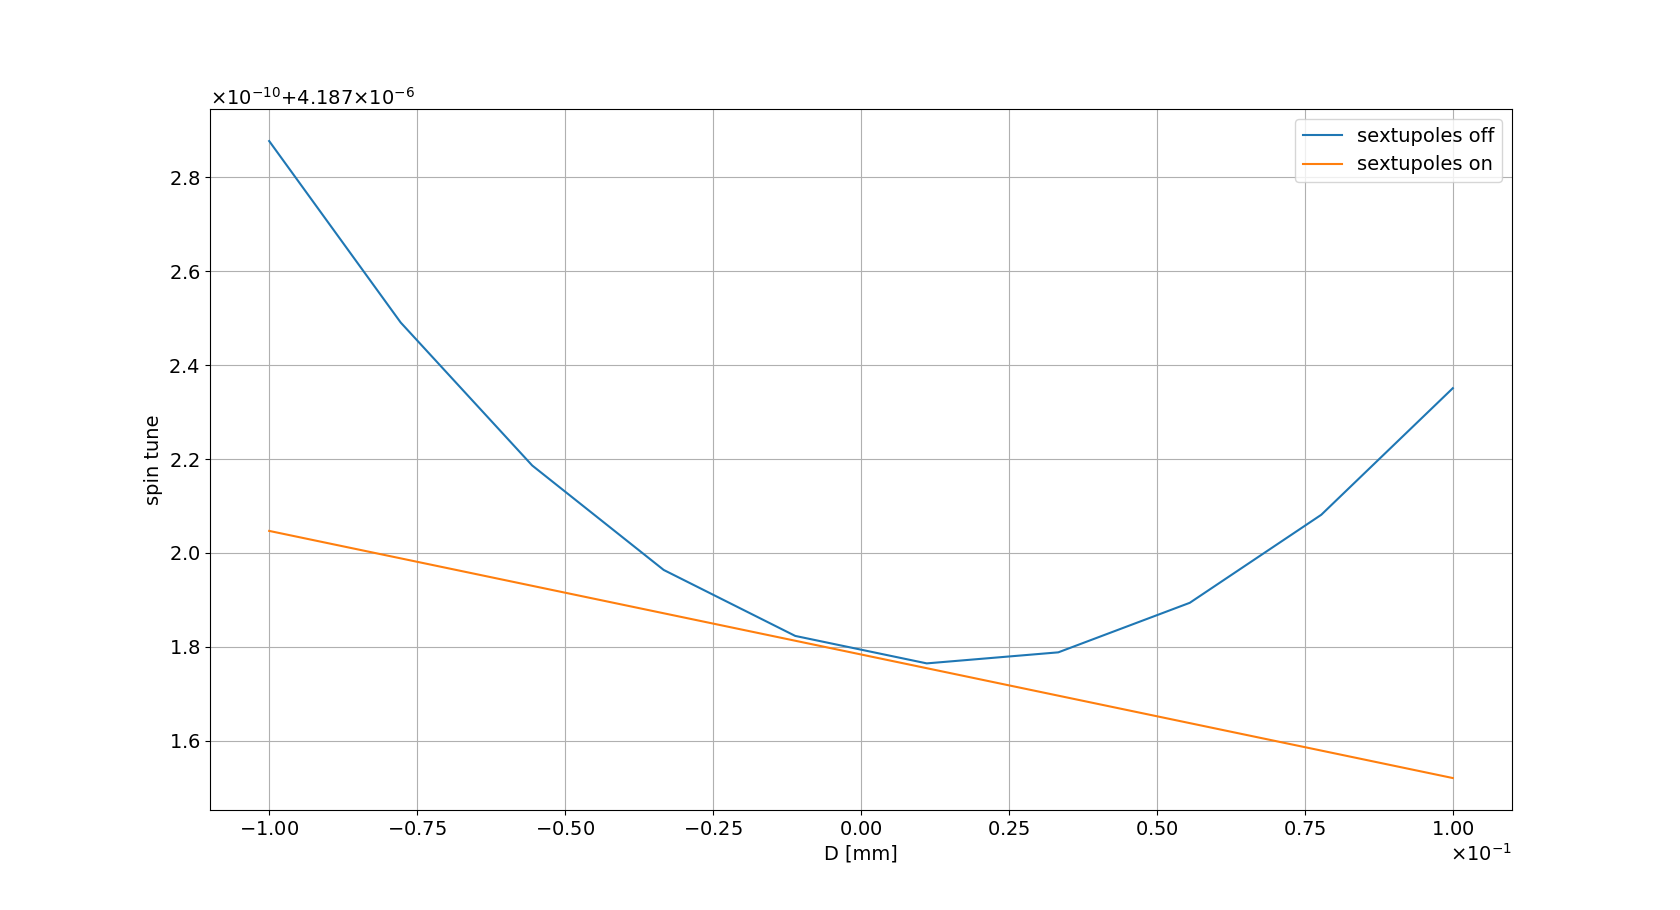
\includegraphics[width=\linewidth]{../img/IPAC19/spin_tune_decoh_d_offset}
    \caption{For particles involved in synchrotron oscillation only.\label{fig:st_decoh_synchrotron}}
  \end{subfigure}
  \caption{Spin tune a as function of initial horizontal, vertical, or momentum offset of the particle,
    with (optimized) and without (unoptimized) correcting sextupoles.\label{fig:decoherence_suppression_sim}}
\end{figure}

\section{Simulation of decohrence in an imperfect lattice}
In this simulation we rotated the E+B elements about the optic axis by angles generated from the
normal distribution $\alpha \sim N(0, 1\cdot 10^{-4})$ rad. The value $\sigma_\alpha = 1\cdot 10^{-4}$ is
a realistic~\cite{Senichev:2017amn} element alignment error standard deviation. A rotation of an E+B element
does not cause a perturbation of the closed orbit, since the net Lorentz force is kept constant.

\begin{figure}[ht]
  \centering
  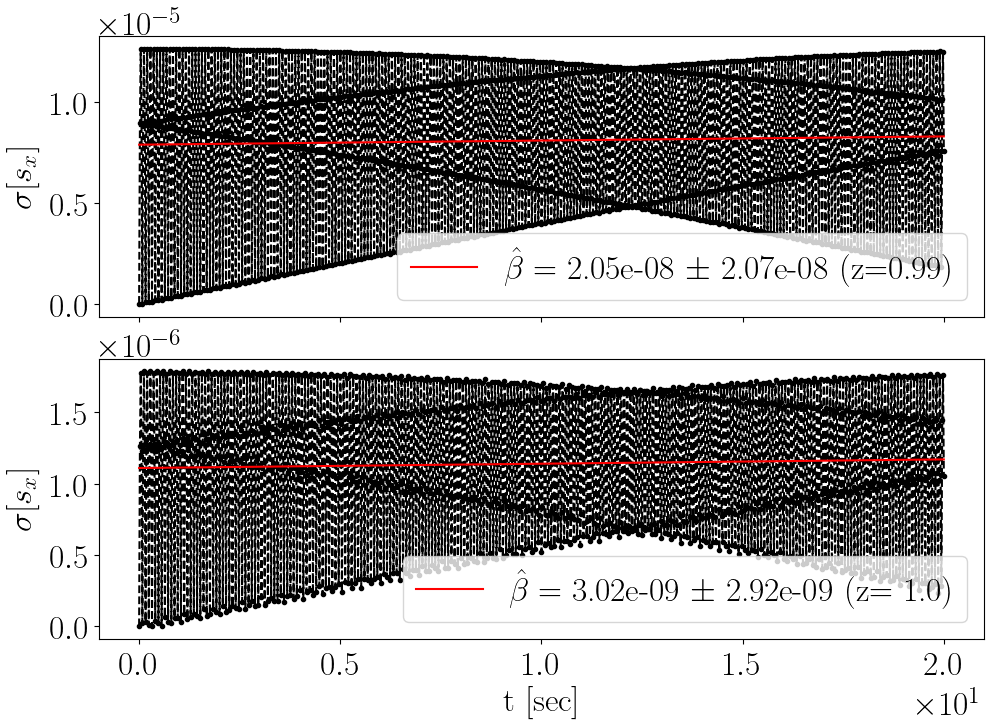
\includegraphics[width=\linewidth]{../img/IPAC19/SX_decoh_20sec_both}
  \caption{Standard deviation of the radial spin vector components in a particle bunch.
    Top panel: sextupoles are turned off; bottom panel: sextupoles are turned on.\label{fig:decoh_rms_sx}}
\end{figure}

Figure~\ref{fig:decoh_rms_sx} shows the standard deviation of the radial spin-vector components in a particle bunch before and after turning on correcting sextupoles. Because an imperfect lattice was used, the particles' spin-vectors precess in the vertical plane at a rapid pace, and hence the RMS-value of $S_x$ is an oscillating function that does not show a long-term growth trend (slope estimate $(2 \pm 2)\cdot 10^{-8}$ 1/sec); there's no decoherence in the horizontal plane. Use of correcting sextupoles further reduces the amplitude of the $\sigma_{S_x}$-oscillations.

\begin{figure}[ht]
  \centering
  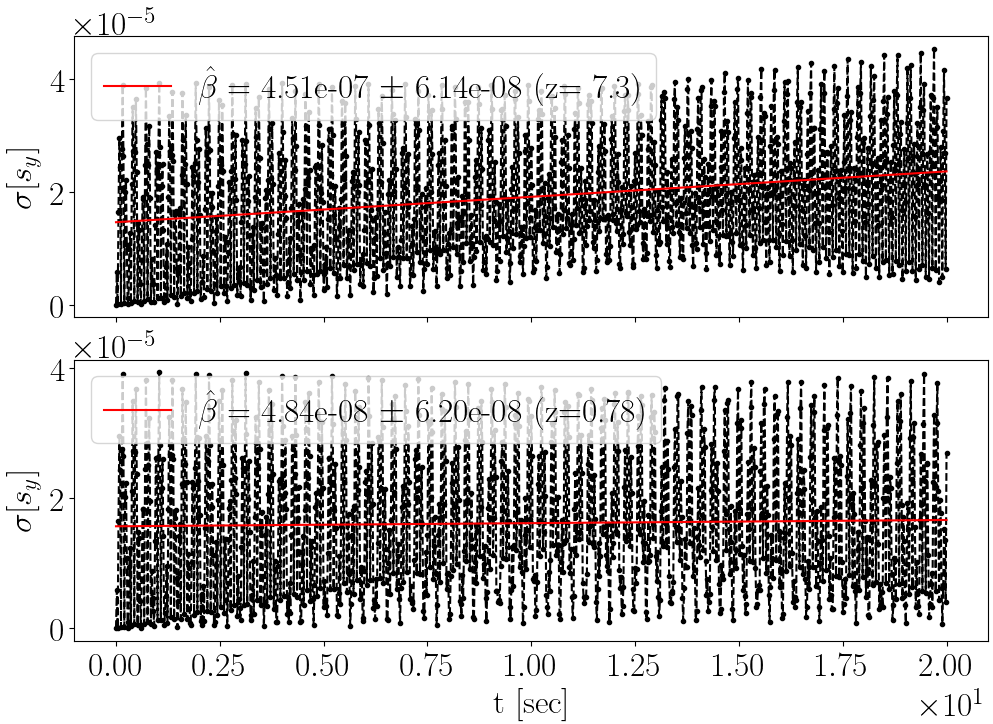
\includegraphics[width=\linewidth]{../img/IPAC19/SY_decoh_20sec_both}
  \caption{Standard deviation of the vertical spin vector components in a particle bunch.
    Top panel: sextupoles are turned off; bottom panel: sextupoles are turned on.\label{fig:decoh_rms_sy}}
\end{figure}

Figure~\ref{fig:decoh_rms_sy} shows the same statistic for the vertical components. One observes a presence of a long-term trend (slope estimate $(4.5 \pm 0.6)\cdot 10^{-7}$ 1/sec) prior to turning on correcting sextupoles (Fig.~\ref{fig:decoh_rms_sy}, top panel). Sextupole correction does not reduce the amplitude of the $\sigma_{S_y}$-oscillations, but it does remove the long-term trend (Fig.~\ref{fig:decoh_rms_sy}, bottom panel,
slope estimate $(5 \pm 6) \cdot 10^{-8}$ 1/sec).

\section{Conclusions}
Spin decoherence is a major problem for any experiment aiming to measure the EDM of an elementary particle
using the storage ring method,~\cite{BNL:Deuteron2008} as it drastically reduces the
possible measurement cycle time. In the present work we have described the mechanism by which it arises,
and a method by which it can be suppressed. We have shown that by means of this method the
parabolic dependence of spin tune on the particle coordinate can be removed. The remaining
linear decoherence effect observed in Fig.~\ref{fig:st_decoh_horizontal} and~\ref{fig:st_decoh_synchrotron}
can likely be suppressed by use of an RF-cavity.~\cite[p.~210]{Eremey:Thesis}

\begin{thebibliography}{9}
  
\bibitem{COSY:SpinTuneMapping}
  A. Saleev et al., (JEDI Collaboration), ``Spin tune mapping as a novel tool to probe
  the spin dynamics in storage rings.'' Phys. Rev. Accel. Beams 20 (2017) no.7, 072801.

\bibitem{Senichev:IPAC13-WEPEA036}
   Y. Senichev, R. Maier, D. Zyuzin, and N. V. Kulabukhova,
   \textquotedblleft{Spin Tune Decoherence Effects in Electro- and Magnetostatic Structures}\textquotedblright,
   in \emph{Proc. 4th Int. Particle Accelerator Conf. (IPAC'13)}, Shanghai, China, May 2013, paper WEPEA036,
   pp. 2579--2581. 

\bibitem{Senichev:2017amn} 
  Y.~Senichev, A.~Aksentev, A.~Ivanov and E.~Valetov,
  %``Frequency domain method of the search for the deuteron electric dipole moment in a storage ring
  %with imperfections,''
  arXiv:1711.06512 [physics.acc-ph].
  %%CITATION = ARXIV:1711.06512;%%

\bibitem{COSY:Website}
  COSY INFINITY, \url{cosyinfinity.org}

\bibitem{BNL:Deuteron2008}
  D. Anastassopoulos et at., (srEDM Collaboration), ``Search for a permanent electric dipole moment of
  the deuteron nucleus at the $10^{-29}~e\cdot cm$ level,'' proposal as submitted to the BNL PAC, April 2008.

\bibitem{Eremey:Thesis}
  E. Valetov, ``Field modeling, symplectic tracking, and spin decoherence for the EDM and muon g-2 lattices,''
  PhD thesis, Dept. of Phys. and Astr., Michigan State University, East Lansing, Michigan, USA.
  %% \url{http://collaborations.fz-juelich.de/ikp/jedi/public_files/theses/valetovphd.pdf}
  
\end{thebibliography}
\end{document}
